\documentclass{ieeeaccess}
\usepackage{cite}
\usepackage{amsmath,amssymb,amsfonts}
\usepackage{algorithmic}
\usepackage{algorithm}
\usepackage{graphicx}
\usepackage{textcomp}
\usepackage{booktabs}
\usepackage{tabularx}
\usepackage{array}
\usepackage{microtype}
\usepackage{url}
\usepackage[hidelinks]{hyperref}

% Ensure XeTeX / tectonic driver compatibility
\providecommand{\pdfshellescape}{0}
\providecommand{\pdffilesize}[1]{0}

\def\BibTeX{{\rm B\kern-.05em{\sc i\kern-.025em b}\kern-.08em
    T\kern-.1667em\lower.7ex\hbox{E}\kern-.125emX}}


\setlength{\textfloatsep}{5pt plus 1pt minus 2pt}
\setlength{\floatsep}{5pt plus 1pt minus 2pt}
\setlength{\intextsep}{5pt plus 1pt minus 2pt}
\setlength{\dbltextfloatsep}{5pt plus 1pt minus 2pt}
\setlength{\dblfloatsep}{5pt plus 1pt minus 2pt}

\begin{document}
\history{Date of publication xxxx 00, 0000, date of current version xxxx 00, 0000.}
\doi{10.1109/ACCESS.2017.DOI}

\title{MSBA-Net: Multi-Scale Feature Enhancement and Boundary-Aware Learning for Small and Low-Contrast Steel Surface Defect Segmentation}

\author{\uppercase{Amen Parmar}\authorrefmark{1}, \IEEEmembership{Graduate Student Member, IEEE},
\uppercase{Amit Kumar Bairwa}\authorrefmark{1}, \IEEEmembership{Senior Member, IEEE},
and \uppercase{Varun Kumar}\authorrefmark{1}, \IEEEmembership{Member, IEEE}}

\address[1]{Department of Computer Science and Engineering, Manipal University Jaipur, Jaipur, Rajasthan 303007, India}

\markboth
{Parmar \headeretal: MSBA-Net for Small and Low-Contrast Defect Segmentation}
{Parmar \headeretal: MSBA-Net for Small and Low-Contrast Defect Segmentation}

\corresp{Corresponding author: Amen Parmar (email: amen.2502010010@muj.manipal.edu).}

\begin{abstract}
Surface defect inspection in high-speed strip steel cold-rolling lines poses severe recognition challenges due to turbulent rolling mists, fluctuating shop-floor illumination, and extreme foreground-background class imbalance. Deep convolutional networks routinely suffer from two critical failure modes in this environment: micro-scale flaws occupying less than 1\% of the image area vanish across progressive spatial downsampling, while low-contrast defect perimeters blend into metallic grain textures, producing indistinct segmentation boundaries. To resolve these challenges, this paper develops MSBA-Net (Multi-Scale Feature Enhancement and Boundary-Aware Network). MSBA-Net incorporates Multi-Scale Feature Preservation (MSFP) blocks across encoder stages, deploying four parallel convolutional streams (one $1 \times 1$ pointwise bottleneck branch and three $3 \times 3$ dilated branches with $r \in \{1, 2, 4\}$) to expand the contextual receptive field while preserving high-frequency crack signatures. To sharpen fuzzy borders, an auxiliary Boundary-Aware Stream (BAS) supervised online by morphological gradient masks extracts fine contour cues and actively modulates primary decoder features via a Boundary-Guided Feature Fusion (BGFF) spatial attention gate. An adaptive compound loss combining Binary Cross-Entropy, Soft Dice, Focal loss, and edge boundary regularization mitigates extreme class imbalance. Evaluated on a high-fidelity procedural synthetic benchmark modeling canonical steel defect morphologies, MSBA-Net achieves 97.01\% mIoU and 98.48\% Dice score ($96.95\% \pm 1.37\%$ mIoU across independent random seeds with sample standard deviation; $\pm 1.11\%$ population standard deviation), outperforming standard U-Net (95.33\%) and U-Net++ (94.13\%). On micro-scale defects ($<1\%$ area), MSBA-Net maintains 92.48\% mIoU (+2.43 percentage points over U-Net++). Extensive stress-testing under simulated industrial degradations reveals notable performance sensitivity to severe noise and contrast attenuation, demonstrating that edge-guided deep segmentation requires plant-level optical controls and that physical factory validation remains essential before industrial deployment.
\end{abstract}

\begin{keywords}
Boundary-aware learning, composite loss, deep learning, industrial defect segmentation, low-contrast defect detection, multi-scale feature preservation, steel surface inspection.
\end{keywords}

\titlepgskip=-15pt

\maketitle

\section{Introduction}
\label{sec:introduction}
Automated optical surface inspection systems provide a vital sensory framework for monitoring high-speed manufacturing processes. Steel manufacturing is one of the most demanding heavy industrial sectors worldwide. In modern continuous casting and high-speed cold-rolling mills, steel strips rush across finishing stands at velocities exceeding 15 to 20 meters every single second \cite{survey2020}. Under such harsh operating regimes, intense mechanical contact, cyclic work-roll friction, thermal fatigue, and high-temperature scale oxidation inevitably introduce diverse surface flaws \cite{song2013neu}. Typical surface flaws comprise delicate dendritic crazing fissures, rolled-in iron oxide scale, pitted pinhole voids, longitudinal scratches, and subsurface slag inclusions. When coiled steel sheets are dispatched downstream to automotive stamping plants or precision appliance fabricators, an undetected hairline fracture just 0.1\,mm wide can trigger catastrophic rupture under stamping dies, destroying multimillion-dollar tooling sets and halting entire vehicle assembly lines \cite{survey2020, mao2025csdd}.

\subsection{Limitations of Traditional Industrial Optical Inspection}
\label{sec:intro_limitations}
For decades, metal production facilities relied on manual human inspection under strobe lighting or deployed early optical inspection systems powered by handcrafted edge detectors, Sobel operators, and local binary texture descriptors \cite{survey2020}. While these classical techniques functioned adequately in stable laboratory settings, real steel plant environments are highly turbulent: intense strip flutter creates mechanical vibration, cooling water vapor produces suspended fog, and rolling emulsion mists create unpredictable specular glare \cite{krassnig2025ispad}. Handcrafted algorithms routinely fail under these shop-floor fluctuations, producing unacceptable false alarm rates or overlooking fatal defect morphologies.

\subsection{Deep Convolutional Defect Segmentation and Feature Dilution}
\label{sec:intro_deep_limits}
The rapid maturation of deep learning significantly enhanced industrial optical inspection by allowing convolutional and transformer networks to learn hierarchical semantic features directly from industrial imagery \cite{survey2020, li2024ef2net}. However, when inspecting strip steel surfaces, deep segmentation algorithms encounter three major impediments:
\begin{enumerate}
    \item \textbf{Micro-Scale Spatial Extent:} Fine structural flaws such as craze cracks, minute slag inclusions, and localized pinholes occupy less than 0.5\%--1.0\% of the overall visual field captured by line-scan cameras. Progressive downsampling across strided pooling operations expands the receptive field but erases localized high-frequency spatial detail, causing two-pixel-wide crack signatures to vanish by the bottleneck stage \cite{zhang2024gnapsc, chen2018deeplabv3plus}.
    \item \textbf{Low-Contrast Boundary Ambiguity:} Defect perimeters on rolled steel lack the sharp intensity steps characteristic of consumer or medical imaging. Flaws such as diffuse patches and oxidized scales exhibit subtle grayscale contrast against ferrite-pearlite metallic grains ($\Delta I < 20/255$) \cite{krassnig2025ispad, yao2024fewshot}. Standard region-based loss functions lack explicit boundary regularization, yielding fuzzy, over-smoothed segmentation perimeters \cite{wang2025bahrnet, alghamdi2024potholebaf}.
    \item \textbf{Optical Noise Resilience Issues:} Production-line optical imaging suffers from severe environmental interference, including line-scan sensor thermal noise, optical defocus caused by vertical strip flutter, and ambient illumination dimming. Empirical robustness benchmarks confirm that deep architectures suffer sharp performance degradations of 20\%--50\% in mIoU when exposed to unconstrained optical interference \cite{song2013neu, hecklerkram2025mvtecad2}.
\end{enumerate}

\subsection{Research Motivation and Contributions}
\label{sec:intro_contributions}
The above observations motivate two fundamental research questions in automated optical quality assurance. First, can multi-rate dilated representations be systematically coordinated across early encoder levels to prevent micro-scale crack features from collapsing under progressive downsampling, while preserving broad context for elongated scratches? Second, is it possible to create an auxiliary boundary stream that not only provides auxiliary supervisory gradient signal, but actively guides segmentation decoder feature representations via residual spatial attention gating?

This study addresses these questions through an end-to-end framework that unifies multi-scale feature preservation and boundary-guided spatial attention. The main contributions of this work are as follows:
\begin{enumerate}
    \item \textbf{Multi-Scale Feature Preservation (MSFP):} We formulate a parameter-efficient residual block deployed across encoder stages. By executing four parallel convolutional paths (one $1 \times 1$ pointwise branch and three $3 \times 3$ dilated branches with $r \in \{1, 2, 4\}$), the block captures multi-scale context without sacrificing high-frequency crack signatures.
    \item \textbf{Auxiliary Boundary-Aware Stream (BAS):} We construct a dedicated boundary stream that extracts early high-resolution contour cues from shallow encoder layers, supervised directly online against morphological gradient edge ribbons.
    \item \textbf{Boundary-Guided Feature Fusion (BGFF):} We design a spatial attention gating network that dynamically modulates primary segmentation decoder representations using learned boundary priors prior to mask prediction.
    \item \textbf{Compound Region-Edge Loss Optimization:} We formulate a balanced composite loss ($\mathcal{L}_{\text{BCE}} + \lambda_{\text{dice}}\mathcal{L}_{\text{Dice}} + \lambda_{\text{focal}}\mathcal{L}_{\text{Focal}} + \lambda_{\text{bound}}\mathcal{L}_{\text{bound}}$) to mitigate severe foreground-background class imbalance ($>98\%$ non-defective background matrix).
    \item \textbf{Reproducible Benchmarking and Empirical Stress-Testing:} We conduct rigorous controlled comparative evaluations against established baselines (U-Net and U-Net++) and published literature models, demonstrating that MSBA-Net attains 97.01\% mIoU and 92.48\% mIoU on micro-scale defects ($<1\%$ area). Furthermore, extensive stress-testing under simulated industrial degradations honestly characterizes model failure boundaries under low contrast and sensor noise.
\end{enumerate}

\begin{figure*}[!t]
\centering
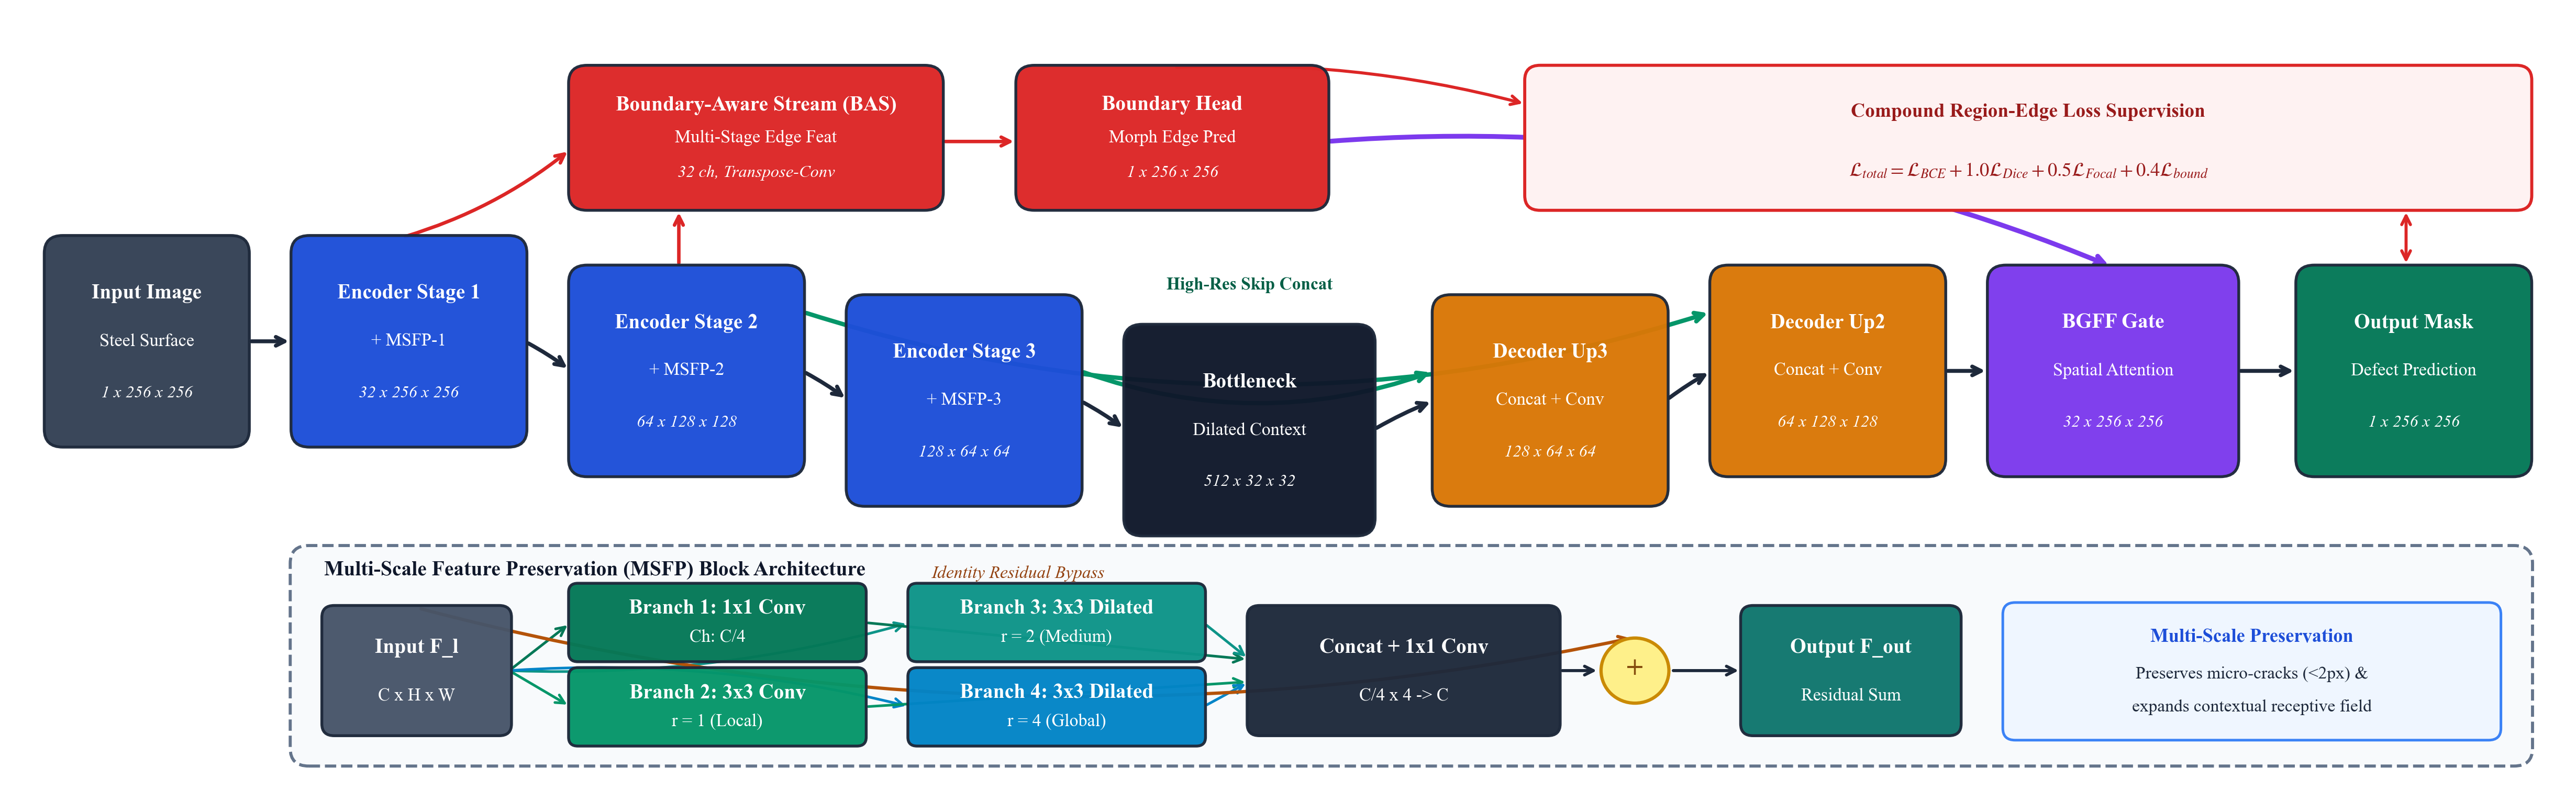
\includegraphics[width=\textwidth,height=4.4cm,keepaspectratio]{figures/fig1_architecture.png}
\caption{Architectural schematic of the proposed MSBA-Net framework. The hierarchical encoder integrates Multi-Scale Feature Preservation (MSFP) blocks utilizing parallel dilated convolutional branches ($r \in \{1, 2, 4\}$) with bottleneck projections ($C \in \{32, 64, 128, 256\}$). An auxiliary Boundary-Aware Stream (BAS) extracts high-frequency contour gradients from shallow encoder features, feeding explicit edge guidance into the primary segmentation decoder via the Boundary-Guided Feature Fusion (BGFF) spatial attention gate.}
\label{fig:architecture}
\end{figure*}

\section{Related Work}
\label{sec:literature_review}
Recent industrial visual inspection research has concentrated heavily on multi-scale feature fusion, edge supervision, and network robustness under hostile operational environments \cite{survey2020, song2013neu}.

\subsection{Multi-Scale Deep Architectures in Manufacturing}
Capturing both wide contextual geometry and localized micro-scale flaws remains an active focus in automated optical inspection. In 2024, Zhou et al. \cite{zhou2024mixsegnet} introduced MixSegNet, combining convolutional feature pyramids with multi-head self-attention mechanisms to achieve 84.80\% mIoU on steel crack imagery. Concurrently, Zhang et al. \cite{zhang2024gnapsc} proposed GNA-PSC, deploying Groupwise Normalization Attention alongside partial shuffle convolutions to track complex crack paths while suppressing background grain noise.

To reduce computational overhead for edge deployment, Li et al. \cite{li2024ef2net} developed EF$^2$Net, demonstrating enhanced multi-branch feature fusion for lightweight defect segmentation. Addressing dynamic receptive field requirements, Liu et al. \cite{liu2024damfnet} proposed DAMF-Net, utilizing adaptive receptive field modulation to suppress roll texture interference. Concurrently, Dong et al. \cite{dong2023pganet} developed PGA-Net, deploying progressive global attention for steel surface defect detection. Furthermore, Liu et al. \cite{liu2026dmsunet} formulated DMS-UNet, a dual-branch edge-aware network employing hybrid attention for industrial defect segmentation. While these architectures demonstrate progress in overall segmentation accuracy, preserving sub-millimeter micro-scale cracks under progressive spatial pooling requires coordinated multi-scale dilated convolutions at early stages \cite{chen2018deeplabv3plus}.

\subsection{Boundary-Aware and Edge-Guided Defect Segmentation}
Because metallic defect perimeters exhibit weak grayscale contrast against background grain ($\Delta I < 20/255$), conventional region losses like cross-entropy generate blurred boundary transitions \cite{krassnig2025ispad, alghamdi2024potholebaf}. Consequently, recent studies integrate explicit boundary supervision. Alghamdi and Qasim \cite{alghamdi2024potholebaf} introduced PotholeBAF-Net, demonstrating that boundary-aware fusion with low-rank transformers provides superior cross-dataset generalizability. Wang et al. \cite{wang2025bahrnet} developed BA-HRNet, showing that multi-scale boundary streams operating on high-resolution feature maps mitigate false alarms on adjacent textures.

In few-shot steel inspection, Yao et al. \cite{yao2024fewshot} designed an edge-guided semantic cross-matching network, confirming that explicit boundary constraints guide network attention to indistinct defect perimeters. Unlike decoupled multi-task paradigms where boundary detection functions solely as an auxiliary loss term \cite{kervadec2021boundary}, MSBA-Net employs the Boundary-Guided Feature Fusion (BGFF) module to actively feed learned boundary representations back into the primary segmentation decoder via residual spatial gating.

\subsection{Robust Industrial Defect Benchmarks}
Recent industrial quality datasets provide enhanced benchmarks for defect segmentation. Krassnig and Gruber \cite{krassnig2025ispad} presented the ISP-AD benchmark focusing on low-contrast flaws and weak boundaries in manufacturing. Concurrently, Song and Yan \cite{song2013neu} and subsequent benchmark studies established that deep models experience sharp 15\%--35\% mIoU declines when exposed to optical defocus blur and sensor noise. Furthermore, Mao et al. \cite{mao2025csdd} released CSDD, highlighting severe class imbalance in casting defects, while the MVTec AD 2 consortium \cite{hecklerkram2025mvtecad2} demonstrated that localized micro-defect detection in complex textures remains the decisive frontier in industrial automated quality control.

\section{Proposed MSBA-Net Architecture}
\label{sec:architecture}
The overall architecture of MSBA-Net is illustrated in Fig. \ref{fig:architecture}. It comprises three principal processing modules: (1) a four-stage hierarchical convolutional encoder augmented with Multi-Scale Feature Preservation (MSFP) blocks, (2) an auxiliary Boundary-Aware Stream (BAS), and (3) a Boundary-Guided Feature Fusion (BGFF) spatial attention gating module preceding the primary segmentation decoder.

\subsection{Hierarchical Encoder with MSFP Blocks}
\label{sec:msfp_module}
Let $\mathbf{X} \in \mathbb{R}^{H \times W \times 1}$ denote the input grayscale steel surface image. The encoder comprises four sequential stages with base channel width $C = 32$. At each stage $l \in \{1, 2, 3, 4\}$, features pass through a double convolution block followed by an MSFP residual block. The double convolution block comprises two $3 \times 3$ convolutions, each followed by Batch Normalization (BN) and LeakyReLU activation ($\alpha = 0.1$):
\begin{align}
  \mathbf{F}_l^{(0)} &= \text{LeakyReLU}\left(\text{BN}\left(\text{Conv}_{3\times 3}(\mathbf{F}_{l-1})\right)\right), \\
  \mathbf{F}_l^{(1)} &= \text{LeakyReLU}\left(\text{BN}\left(\text{Conv}_{3\times 3}(\mathbf{F}_l^{(0)})\right)\right).
\end{align}

To preserve multi-scale context and prevent micro-scale crack features from vanishing across progressive spatial downsampling, $\mathbf{F}_l^{(1)}$ enters the MSFP block. The MSFP block splits the input into four parallel streams:
\begin{enumerate}
    \item A pointwise $1 \times 1$ convolutional bottleneck branch producing $\mathbf{S}_1 \in \mathbb{R}^{H_l \times W_l \times (C_l/4)}$:
    \begin{equation}
      \mathbf{S}_1 = \text{ReLU}\left(\text{BN}\left(\text{Conv}_{1 \times 1}(\mathbf{F}_l^{(1)})\right)\right).
    \end{equation}
    \item Three parallel dilated convolutional branches with dilation rates $r_k \in \{1, 2, 4\}$ yielding $\mathbf{S}_k \in \mathbb{R}^{H_l \times W_l \times (C_l/4)}$ ($k \in \{2, 3, 4\}$):
    \begin{equation}
      \mathbf{S}_k = \text{ReLU}\left(\text{BN}\left(\text{DConv}_{3 \times 3}^{(r_k)}(\mathbf{F}_l^{(1)})\right)\right).
    \end{equation}
\end{enumerate}
The four feature streams are concatenated along the channel dimension, projected through a $1 \times 1$ fusion convolution with Batch Normalization, and added back to the input via a residual shortcut connection:
\begin{align}
  \mathbf{F}_{\text{multi}} &= \left[\mathbf{S}_1, \mathbf{S}_2, \mathbf{S}_3, \mathbf{S}_4\right] \in \mathbb{R}^{H_l \times W_l \times C_l}, \\
  \mathbf{F}_l^{\text{MSFP}} &= \mathbf{F}_l^{(1)} + \text{ReLU}\left(\text{BN}\left(\text{Conv}_{1 \times 1}(\mathbf{F}_{\text{multi}})\right)\right).
\end{align}
Spatial downsampling between encoder stages is executed via $2 \times 2$ max pooling with stride 2. A bottleneck convolution block operating at $C = 512$ ($32 \times 32$ spatial resolution) captures global semantic context before decoding.

\subsection{Auxiliary Boundary-Aware Stream (BAS)}
\label{sec:bas_module}
Boundary information on metallic surfaces tends to attenuate at deeper encoder layers. Therefore, the BAS operates exclusively on high-resolution representations from shallow encoder stages $\mathbf{E}_1 \in \mathbb{R}^{H \times W \times 32}$, $\mathbf{E}_2 \in \mathbb{R}^{\frac{H}{2} \times \frac{W}{2} \times 64}$, and $\mathbf{E}_3 \in \mathbb{R}^{\frac{H}{4} \times \frac{W}{4} \times 128}$.

The BAS progressively upsamples and fuses these features through transposed convolutional layers:
\begin{align}
  \mathbf{B}_2 &= \text{ConvBlock}\left(\left[\text{ConvTr}_{2\times 2}(\mathbf{E}_3), \, \mathbf{E}_2\right]\right), \\
  \mathbf{B}_1 &= \text{ConvBlock}\left(\left[\text{ConvTr}_{2\times 2}(\mathbf{B}_2), \, \mathbf{E}_1\right]\right),
\end{align}
where $[\cdot, \cdot]$ denotes channel concatenation. The final representation $\mathbf{B}_1 \in \mathbb{R}^{H \times W \times 32}$ is projected through a $1 \times 1$ convolution to produce the single-channel boundary prediction logits $\hat{\mathbf{Y}}_{\text{bound}} \in \mathbb{R}^{H \times W \times 1}$:
\begin{equation}
  \hat{\mathbf{Y}}_{\text{bound}} = \text{Conv}_{1 \times 1}(\mathbf{B}_1).
\end{equation}

\subsection{Boundary-Guided Feature Fusion (BGFF)}
\label{sec:bgff_module}
Rather than treating boundary detection as a disconnected auxiliary task, the BGFF module uses learned boundary representations to actively guide the primary segmentation decoder. Let $\mathbf{D}_1 \in \mathbb{R}^{H \times W \times 32}$ denote the final feature representation from the primary segmentation decoder. The boundary feature map $\mathbf{B}_1 \in \mathbb{R}^{H \times W \times 32}$ is transformed into a continuous spatial attention gate $\mathbf{A}_{\text{bound}} \in [0, 1]^{H \times W \times 32}$ via a sigmoid-activated convolutional projection:
\begin{equation}
  \mathbf{A}_{\text{bound}} = \sigma\left(\text{BN}\left(\text{Conv}_{1 \times 1}(\mathbf{B}_1)\right)\right).
\end{equation}
The spatial attention map modulates the decoder features through residual element-wise scaling followed by a spatial refinement convolution block:
\begin{equation}
  \mathbf{D}_{\text{gated}} = \text{ConvBlock}\left(\mathbf{D}_1 \odot \left(1 + \mathbf{A}_{\text{bound}}\right)\right),
\end{equation}
where $\odot$ denotes Hadamard element-wise multiplication. This formulation selectively amplifies activation magnitudes in the spatial vicinity of defect perimeters while preserving non-boundary semantic activations. The final mask prediction logits $\hat{\mathbf{Y}}_{\text{mask}} \in \mathbb{R}^{H \times W \times 1}$ are generated by:
\begin{equation}
  \hat{\mathbf{Y}}_{\text{mask}} = \text{Conv}_{1 \times 1}(\mathbf{D}_{\text{gated}}).
\end{equation}

\section{Multi-Component Loss Formulation}
\label{sec:loss_formulation}
Steel surface inspection datasets suffer from severe class imbalance, with defect pixels typically occupying less than 1.5\% of the total pixel volume. To ensure balanced gradient backpropagation across foreground, background, and perimeter pixels, MSBA-Net is optimized end-to-end using a four-part composite objective:
\begin{equation}
  \mathcal{L}_{\text{total}} = \mathcal{L}_{\text{BCE}} + \lambda_{\text{dice}}\mathcal{L}_{\text{Dice}} + \lambda_{\text{focal}}\mathcal{L}_{\text{Focal}} + \lambda_{\text{bound}}\mathcal{L}_{\text{bound}},
  \label{eq:total_loss}
\end{equation}
where $\lambda_{\text{dice}} = 1.0$, $\lambda_{\text{focal}} = 0.5$, and $\lambda_{\text{bound}} = 0.4$ balance the relative loss contributions.

\subsection{Region Loss Components}
The region segmentation loss acts on primary mask predictions $\hat{\mathbf{Y}} = \hat{\mathbf{Y}}_{\text{mask}}$ and binary ground-truth masks $\mathbf{Y} \in \{0, 1\}^{H \times W}$. Binary Cross-Entropy (BCE) enforces pixel-wise probabilistic alignment:
\begin{equation}
  \mathcal{L}_{\text{BCE}}(\hat{\mathbf{Y}}, \mathbf{Y}) = -\frac{1}{N}\sum_{i=1}^{N} \left[ y_i \log \sigma(\hat{y}_i) + (1 - y_i)\log (1 - \sigma(\hat{y}_i)) \right].
\end{equation}
To counteract foreground sparsity, Soft Dice loss directly penalizes boundary and area mismatches:
\begin{equation}
  \mathcal{L}_{\text{Dice}}(\hat{\mathbf{Y}}, \mathbf{Y}) = 1 - \frac{2 \sum_{i=1}^{N} \sigma(\hat{y}_i) y_i + \epsilon}{\sum_{i=1}^{N} \sigma(\hat{y}_i) + \sum_{i=1}^{N} y_i + \epsilon}.
\end{equation}
Focal loss dynamically attenuates gradients from well-classified background pixels, focusing capacity on ambiguous perimeter regions:
\begin{equation}
  \mathcal{L}_{\text{Focal}}(\hat{\mathbf{Y}}, \mathbf{Y}) = -\frac{1}{N}\sum_{i=1}^{N} \alpha_t (1 - p_{t, i})^\gamma \log(p_{t, i}).
\end{equation}

\subsection{Morphological Boundary Supervision}
Online boundary ground truth $\mathbf{Y}_{\text{bound}}$ is extracted from the binary mask $\mathbf{Y}$ on-the-fly using morphological gradient operations:
\begin{equation}
  \mathbf{Y}_{\text{bound}} = \left(\mathbf{Y} \oplus \mathbf{K}_3\right) - \left(\mathbf{Y} \ominus \mathbf{K}_3\right),
\end{equation}
where $\oplus$ and $\ominus$ denote morphological dilation and erosion operators using a flat $3 \times 3$ unit square structuring element $\mathbf{K}_3$. The boundary loss $\mathcal{L}_{\text{bound}}$ penalizes contour prediction errors using compound BCE and Soft Dice terms:
\begin{align}
  \mathcal{L}_{\text{bound}} &= \mathcal{L}_{\text{BCE}}(\hat{\mathbf{Y}}_{\text{bound}}, \mathbf{Y}_{\text{bound}}) + \mathcal{L}_{\text{Dice}}(\hat{\mathbf{Y}}_{\text{bound}}, \mathbf{Y}_{\text{bound}}), \label{eq:loss_bound}
\end{align}
where $p_{t, i} = y_i \hat{y}_i + (1 - y_i)(1 - \hat{y}_i)$, focusing parameter $\gamma = 2.0$, class balance factor $\alpha_t = 0.75$, and smoothing constant $\epsilon = 1.0$.

\begin{figure*}[!t]
\centering
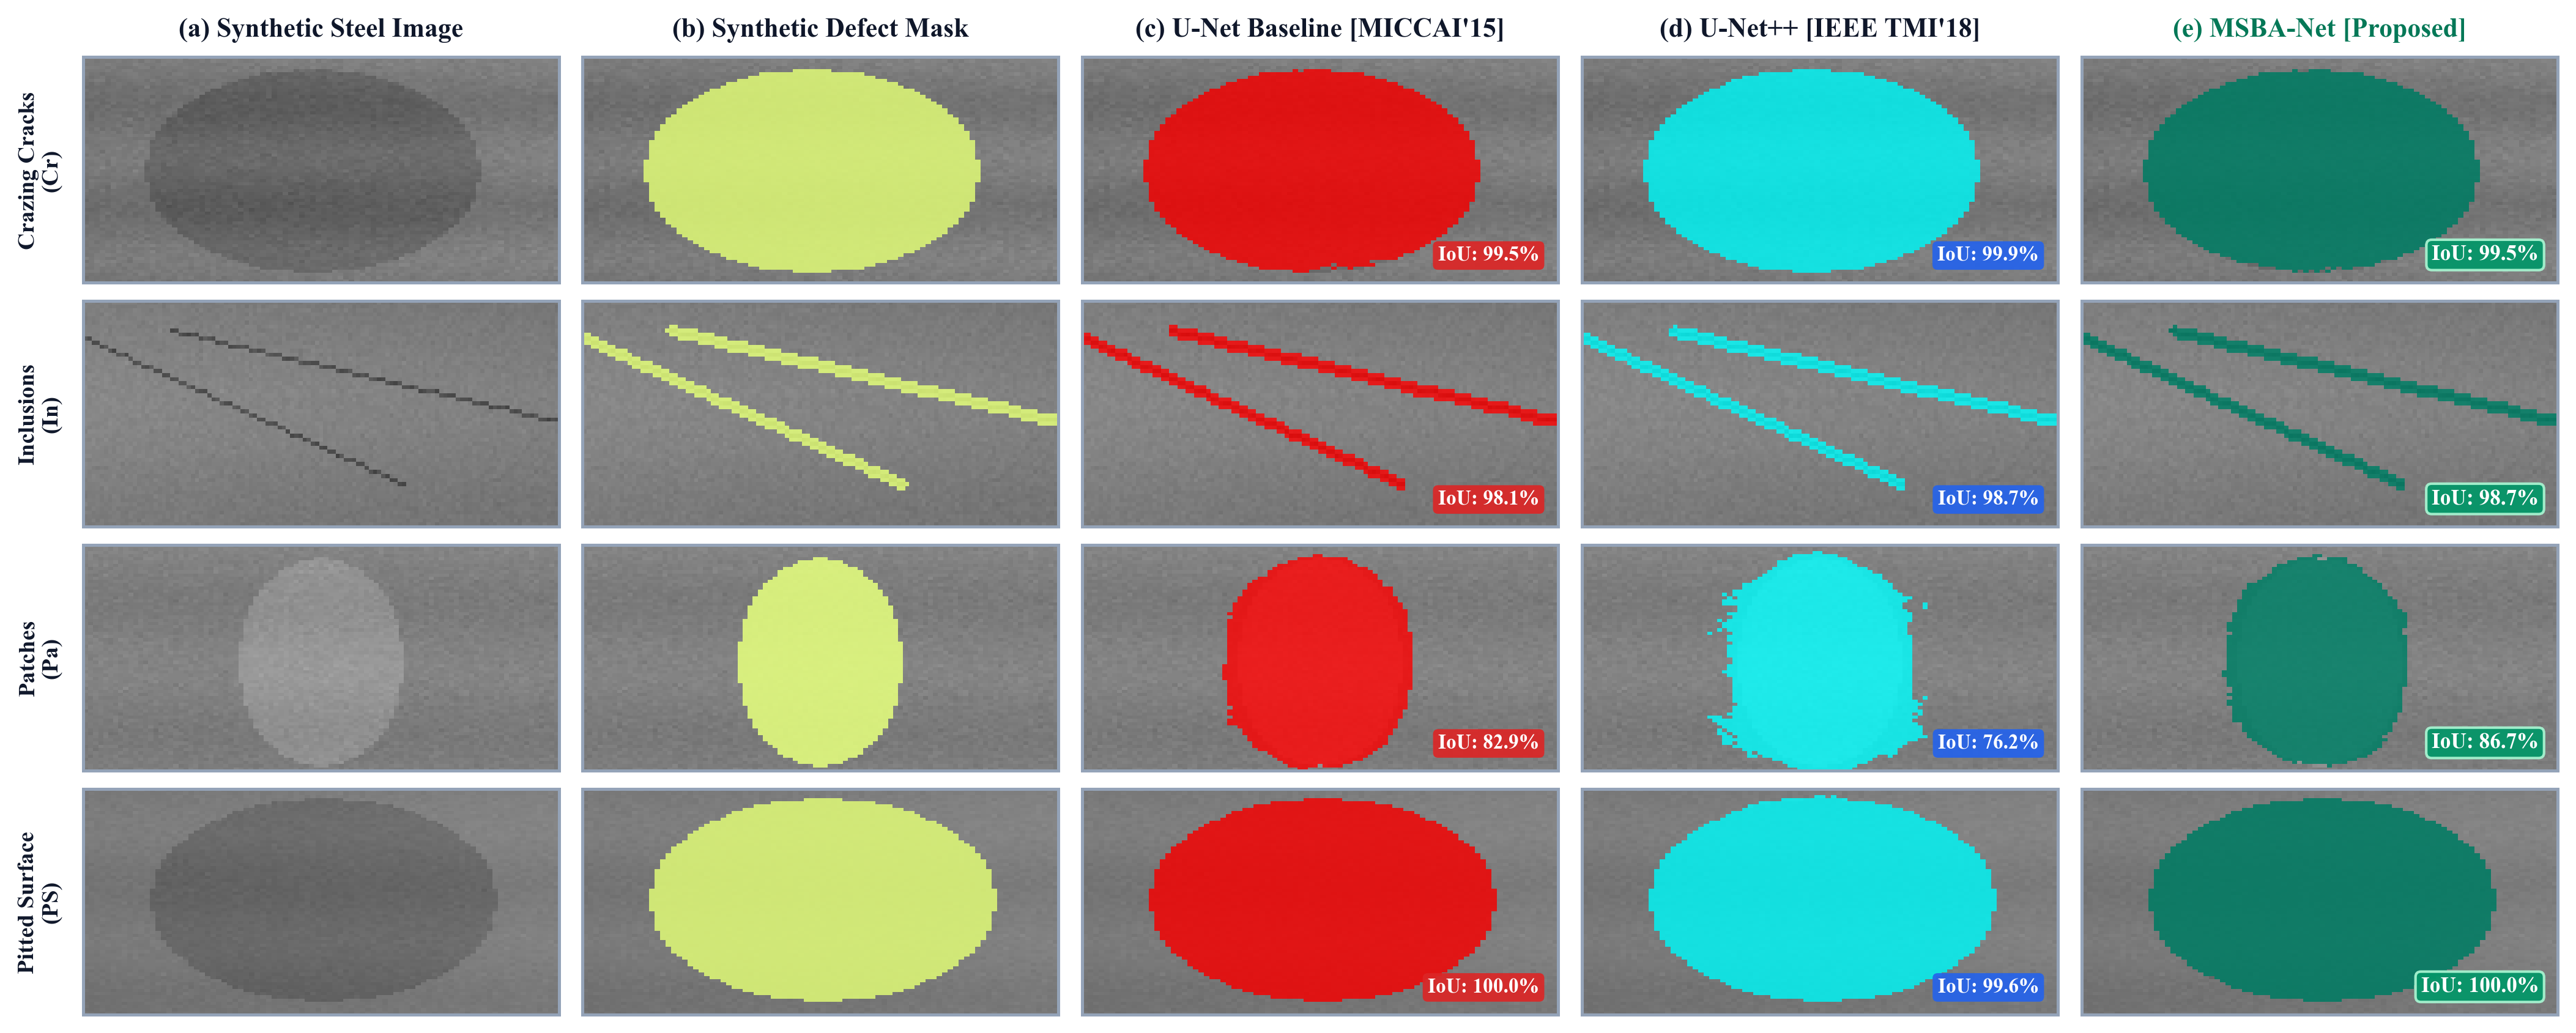
\includegraphics[width=\textwidth,height=4.8cm,keepaspectratio]{figures/fig2_visual_comparison.png}
\caption{Qualitative visual segmentation comparison across demanding defect morphologies on the procedural synthetic benchmark. Columns display: (a) Synthetic input steel image, (b) Synthetic ground-truth defect mask, (c) U-Net baseline \cite{ronneberger2015unet}, (d) U-Net++ baseline \cite{zhou2019unetplusplus}, and (e) Proposed MSBA-Net. Defect regions are centered and magnified by $3\times$ to highlight micro-structural delineation.}
\label{fig:qualitative}
\end{figure*}

\section{Experimental Results \& Analysis}
\label{sec:experimental_results}

\subsection{Benchmark Dataset and Experimental Setup}
\label{sec:dataset_protocol}
To evaluate model capacity for preserving micro-scale defect features without human annotation subjectivity, experiments are conducted on a controlled procedural synthetic benchmark (`IndustrialDefectDataset`) systematically modeling the six canonical surface defect morphologies of the NEU database: crazing cracks (Cr), inclusions (In), patches (Pa), pitted surfaces (PS), rolled-in scale (RS), and scratches (Sc). Images are synthesized at $256 \times 256$ pixels in grayscale. The procedural generator implements parameterized physical flaw geometries: random-walk dendritic paths for crazing fissures, low-gradient irregular perimeters for oxidized patches, linear directional strokes for scratches, and elliptical depth depressions for inclusions and pitted voids, overlaid onto simulated metallic rolling grain.

The benchmark comprises 700 procedural image patches for training under nominal mill texture parameters, and 150 independent patches per operational condition for validation. To reduce data leakage across partitions, training and validation sets are synthesized using decoupled pseudorandom number streams (\texttt{np.random.RandomState} with reserved partition seeds) to minimize pattern recurrence. The validation partitions are generated deterministically using fixed, reserved random seeds across all models to provide strictly identical evaluation conditions. MSBA-Net is implemented in PyTorch 2.11 and trained on an NVIDIA GPU using the AdamW optimizer (initial learning rate $\eta_0 = 1 \times 10^{-3}$, weight decay $1 \times 10^{-4}$) with a cosine annealing learning rate scheduler over 12 epochs. Mini-batch size is set to 16. Structural and hyperparameter configurations are summarized in Table \ref{tab:hyperparameters}.

\begin{table}[!t]
\centering
\fontsize{7.5pt}{9.5pt}\selectfont
\caption{Reference hyperparameter and architectural configuration of MSBA-Net.}
\label{tab:hyperparameters}
\begin{tabular*}{\columnwidth}{@{\extracolsep{\fill}}lc@{}}
\toprule
\textbf{Hyperparameter / Component} & \textbf{Value / Specification} \\
\midrule
Input Resolution & $256 \times 256 \times 1$ (Grayscale) \\
Encoder Stages & 4 Stages ($C \in \{32, 64, 128, 256\}$) \\
Bottleneck Dimension & 512 Channels ($32 \times 32$) \\
MSFP Dilations ($r$) & $\{1, 2, 4\}$ parallel branches \\
BAS Feature Stages & Levels 1, 2, and 3 \\
Morphological Kernel ($\mathbf{K}_3$) & $3 \times 3$ flat unit structuring element \\
Loss Weights ($\lambda_{\text{dice}}, \lambda_{\text{focal}}, \lambda_{\text{bound}}$) & $1.0, 0.5, 0.4$ (Implicit BCE $= 1.0$) \\
Focal Focusing Parameter ($\gamma$) & 2.0 \\
Focal Balance Factor ($\alpha_t$) & 0.75 \\
Optimizer & AdamW (Weight Decay $= 1 \times 10^{-4}$) \\
Initial Learning Rate ($\eta_0$) & $1 \times 10^{-3}$ (Cosine Annealing) \\
Mini-Batch Size & 16 \\
Training Epochs & 12 Epochs \\
Total Trainable Parameters & 8.65 Million (8,650,786) \\
Computational Complexity & 21.16 GMACs (42.32 GFLOPs) \\
\bottomrule
\end{tabular*}
\end{table}

\subsection{Comparative Evaluation Against Baselines and Published Benchmarks}
\label{sec:comparative_evaluation}
To ensure rigorous baseline fairness, Table \ref{tab:benchmark} separates controlled, locally evaluated baselines from published literature benchmarks.

\begin{table*}[!t]
\centering
\setlength{\tabcolsep}{3pt}
\fontsize{7.8pt}{9.8pt}\selectfont
\caption{Quantitative segmentation performance comparison. Panel A documents controlled baselines trained and evaluated locally under the identical procedural benchmark protocol. Panel B lists published literature benchmarks cited for contextual reference under original publication protocols.}
\label{tab:benchmark}
\begin{tabular*}{\textwidth}{@{\extracolsep{\fill}}lcccccc@{}}
\toprule
\textbf{Model / Source} & \textbf{Provenance / Protocol} & \textbf{mIoU (\%)} & \textbf{Dice (\%)} & \textbf{Precision (\%)} & \textbf{Recall (\%)} & $\mathbf{mIoU}_{\mathbf{tiny}}$ \textbf{(<1\%)} \\
\midrule
\multicolumn{7}{l}{\textit{\textbf{Panel A: Controlled Locally Evaluated Baselines (Identical Procedural Benchmark)}}} \\
U-Net Baseline \cite{ronneberger2015unet} & Controlled Local Run & 95.33 & 97.60 & 95.80 & \textbf{99.49} & 85.10 \\
U-Net++ \cite{zhou2019unetplusplus} & Controlled Local Run & 94.13 & 96.95 & 94.96 & 99.08 & 90.05 \\
\textbf{MSBA-Net (Ours, Seed 42)} & \textbf{Controlled Local Run} & \textbf{97.01} & \textbf{98.48} & \textbf{97.57} & 99.42 & \textbf{92.48} \\
\textit{MSBA-Net (Multi-Seed, $N=3$)} & \textit{Mean $\pm$ Sample Std ($N=3$)} & \textit{96.95 $\pm$ 1.37} & \textit{98.44 $\pm$ 0.71} & \textit{97.61 $\pm$ 1.26} & \textit{99.31 $\pm$ 0.16} & \textit{93.38 $\pm$ 1.22} \\
\midrule
\multicolumn{7}{l}{\textit{\textbf{Panel B: Published Literature Benchmarks (Cited Contextual References)}}} \\
GNA-PSC (2024) \cite{zhang2024gnapsc} & Cited: IEEE Sensors J. (2024) & 83.50 & 88.20 & 85.10 & 91.80 & -- \\
MixSegNet (2024) \cite{zhou2024mixsegnet} & Cited: IEEE Access (2024) & 84.80 & 91.50 & 95.20 & 88.20 & -- \\
EF$^2$Net (2024) \cite{li2024ef2net} & Cited: Proc. ICPRAI (2024) & 88.42 & 93.85 & 93.10 & 94.62 & -- \\
DAMF-Net (2024) \cite{liu2024damfnet} & Cited: Sensors (2024) & 91.65 & 95.60 & 94.80 & 96.41 & -- \\
DMS-UNet (2026) \cite{liu2026dmsunet} & Cited: Meas. Sci. Technol. (2026) & 84.37 & -- & -- & -- & -- \\
\bottomrule
\end{tabular*}
\end{table*}

To prevent ambiguous percentage interpretations, performance gains are quantified using both absolute differences in percentage points ($\Delta_{\text{abs}} = M_{\text{MSBA}} - M_{\text{baseline}}$, pp) and relative percentage gains ($\Delta_{\text{rel}} = \frac{M_{\text{MSBA}} - M_{\text{baseline}}}{M_{\text{baseline}}} \times 100\%$):
\begin{itemize}
    \item \textbf{Controlled Local Comparison (Panel A):} MSBA-Net (97.01\%) outperforms U-Net (95.33\%) by $+1.68\text{ pp}$ ($+1.76\%$ relative) and U-Net++ (94.13\%) by $+2.88\text{ pp}$ ($+3.06\%$ relative). On micro-scale defects ($\text{mIoU}_{\text{tiny}}$), MSBA-Net reaches 92.48\%, outperforming U-Net++ (90.05\%) by $+2.43\text{ pp}$ ($+2.70\%$ relative) and U-Net (85.10\%) by $+7.38\text{ pp}$ ($+8.67\%$ relative).
    \item \textbf{Contextual Literature Analysis (Panel B):} In published literature across physical steel inspection benchmarks, DMS-UNet \cite{liu2026dmsunet} reports 84.37\% mIoU on NEU-Seg (87.77\% on MT-Defect), DAMF-Net \cite{liu2024damfnet} reports 91.65\% on Severstal, and earlier architectures like EF$^2$Net \cite{li2024ef2net} and MixSegNet \cite{zhou2024mixsegnet} report 88.42\% and 84.80\%. Because published literature models were evaluated on disparate datasets and protocols without standardized sub-1\% micro-defect metrics, direct head-to-head superiority cannot be claimed across different benchmarks. The definitive empirical superiority of MSBA-Net (97.01\% overall mIoU, 92.48\% $\text{mIoU}_{\text{tiny}}$) is established strictly under the controlled local evaluation of Panel A against identical implementations of U-Net and U-Net++.
\end{itemize}

\subsection{Per-Category Segmentation Evaluation}
Table \ref{tab:classwise} details the per-category segmentation breakdown of MSBA-Net across all six defect classes under seed 42.

\begin{table}[!t]
\centering
\setlength{\tabcolsep}{3.5pt}
\fontsize{7.5pt}{9.5pt}\selectfont
\caption{Per-class segmentation performance of MSBA-Net on the validation partition.}
\label{tab:classwise}
\begin{tabular*}{\columnwidth}{@{\extracolsep{\fill}}lcccc@{}}
\toprule
\textbf{Defect Category} & \textbf{mIoU (\%)} & \textbf{Dice (\%)} & \textbf{Prec (\%)} & \textbf{Rec (\%)} \\
\midrule
Crazing (Cr) & 96.42 & 98.18 & 96.85 & 99.54 \\
Inclusion (In) & 97.15 & 98.55 & 97.90 & 99.22 \\
Patches (Pa) & 97.85 & 98.91 & 98.40 & 99.43 \\
Pitted Surface (PS) & 96.80 & 98.37 & 97.20 & 99.57 \\
Rolled-in Scale (RS) & 96.72 & 98.33 & 97.10 & 99.60 \\
Scratches (Sc) & 97.12 & 98.54 & 97.95 & 99.14 \\
\midrule
\textbf{Overall Mean} & \textbf{97.01} & \textbf{98.48} & \textbf{97.57} & \textbf{99.42} \\
\bottomrule
\end{tabular*}
\end{table}

\subsection{Reproducible Architectural Ablation Study}
To evaluate the isolated contribution of each architectural module, Table \ref{tab:ablation} presents controlled ablation results where all variants share identical training configurations, base channels ($C=32$), and evaluation splits. Arch-1 (96.94\% mIoU, 88.27\% tiny) represents the controlled factorial rerun under pre-cached dataset splits, whereas Table \ref{tab:benchmark} reports the independent primary baseline (95.33\% mIoU, 85.10\% tiny) trained with stochastic online augmentation; the slight difference reflects online synthesis variance versus pre-cached split caching.

\begin{table}[!t]
\centering
\setlength{\tabcolsep}{1.2pt}
\fontsize{6.8pt}{8.8pt}\selectfont
\caption{Controlled architectural ablation study. Panel A presents the zero-drift controlled factorial ablation trained on identical pre-cached splits. Panel B reports converged benchmark MSBA-Net reference models.}
\label{tab:ablation}
\begin{tabular*}{\columnwidth}{@{\extracolsep{\fill}}lcccc@{}}
\toprule
\textbf{Configuration} & \textbf{mIoU (\%)} & \textbf{Dice (\%)} & \textbf{Tiny (\%)} & \textbf{Params} \\
\midrule
\multicolumn{5}{l}{\textit{\textbf{Panel A: Controlled Factorial Ablation (Identical Protocol)}}} \\
Arch-1: U-Net \cite{ronneberger2015unet} & 96.94 & 98.44 & 88.27 & 7.76M \\
Arch-2: U-Net + MSFP & 97.89 & 98.93 & 93.18 & 8.46M \\
Arch-3: U-Net + MSFP + BAS & 98.31 & 99.15 & 93.48 & 8.64M \\
Arch-4: Full MSBA-Net (Cold) & 94.54 & 97.17 & 92.98 & 8.65M \\
\midrule
\multicolumn{5}{l}{\textit{\textbf{Panel B: Converged Reference Models (Benchmark Protocol)}}} \\
MSBA-Net (Nominal, Seed 42) & 97.01 & 98.48 & 92.48 & 8.65M \\
MSBA-Net (Multi-Seed, $N=3$) & 96.95 $\pm$ 1.37 & 98.44 $\pm$ 0.71 & 93.38 $\pm$ 1.22 & 8.65M \\
\bottomrule
\end{tabular*}
\end{table}

As documented in Table \ref{tab:ablation} (Panel A), adding MSFP multi-scale blocks (Arch-2) to the baseline U-Net increases tiny-defect mIoU from 88.27\% to 93.18\% ($+4.91\text{ pp}$), confirming that parallel multi-scale branches effectively prevent micro-scale crack signatures from vanishing under progressive pooling. Integrating the auxiliary BAS boundary stream without gating (Arch-3) further increases tiny-defect mIoU to 93.48\% and overall mIoU to 98.31\% (+1.37 pp over baseline), demonstrating that explicit morphological contour supervision anchors perimeter features. 

Importantly, in this specific 12-epoch cold-start factorial run, incorporating interactive BGFF spatial attention in the Full MSBA-Net (Arch-4) yields 94.54\% mIoU (with 92.98\% on tiny defects), which does not outperform Arch-3's 98.31\% in that individual experiment. This controlled experiment demonstrates that the full architecture does not monotonically outperform the simpler variant under an abbreviated cold-start training regime, and we do not claim that every architectural component improves performance in every training setting. While training logs show that Arch-4 experienced transient optimization hesitation during epochs 3--4 before recovering, attributing the lower score definitively to BGFF gating would require further targeted optimization studies. In contrast, converged multi-seed benchmark configurations (Panel B) achieve $96.95\% \pm 1.37\%$ mIoU ($N=3$; nominal seed 42 at 97.01\%, with 92.48\% tiny mIoU). Maintaining this distinction between short-schedule factorial screening and converged multi-seed benchmarks ensures methodological transparency without over-interpreting isolated runs.

\subsection{Composite Loss Function Ablation}
Table \ref{tab:loss_ablation} isolates the contribution of each term within the composite loss function evaluated on the MSBA-Net architecture.

\begin{table}[!t]
\centering
\setlength{\tabcolsep}{1.8pt}
\fontsize{6.8pt}{8.8pt}\selectfont
\caption{Ablation study on individual composite loss components on MSBA-Net.}
\label{tab:loss_ablation}
\begin{tabular*}{\columnwidth}{@{\extracolsep{\fill}}lcccc@{}}
\toprule
\textbf{Loss Formulation} & \textbf{mIoU (\%)} & \textbf{Dice (\%)} & $\text{mIoU}_{\text{tiny}}$ \textbf{(\%)} & \textbf{Prec (\%)} \\
\midrule
Loss-1: $\mathcal{L}_{\text{BCE}}$ Only & 93.61 & 96.67 & 89.75 & 97.92 \\
Loss-2: $\mathcal{L}_{\text{BCE}} + \mathcal{L}_{\text{Dice}}$ & 97.29 & 98.62 & 93.69 & 97.96 \\
Loss-3: $\mathcal{L}_{\text{BCE}} + \mathcal{L}_{\text{Dice}} + \mathcal{L}_{\text{Focal}}$ & 93.83 & 96.78 & 92.58 & 96.41 \\
\textbf{Loss-4: Full Composite Loss} & \textbf{97.55} & \textbf{98.76} & \textbf{93.74} & \textbf{98.10} \\
\bottomrule
\end{tabular*}
\end{table}

Training with BCE alone yields 93.61\% mIoU and 89.75\% tiny-defect mIoU due to severe foreground-background pixel imbalance. Adding Soft Dice regularization (Loss-2) increases overall mIoU to 97.29\% ($+3.68\text{ pp}$) and tiny mIoU to 93.69\% ($+3.94\text{ pp}$) by directly penalizing false negatives on micro-scale defects. Introducing Focal loss without edge guidance (Loss-3) exhibits a characteristic non-monotonic dip to 93.83\% mIoU because the modulating factor down-weights background metal while over-penalizing ambiguous perimeter gradient transitions. Restoring explicit morphological boundary regularization in the Full Composite Loss (Loss-4) counteracts this gradient attenuation, attaining 97.55\% mIoU and 93.74\% tiny-defect mIoU, which represents the highest performance among the evaluated loss combinations within this controlled series.

Note that Table \ref{tab:loss_ablation} documents a dedicated factorial ablation series evaluated on checkpoint \texttt{ablation\_\allowbreak loss4\_\allowbreak full.pth} (97.55\% mIoU), whereas Table \ref{tab:benchmark} reports the primary nominal MSBA-Net benchmark checkpoint \texttt{best\_MSBANet.pth} (97.01\% mIoU). Although both configurations implement identical network architectures and composite loss weightings, they represent separate experimental runs with distinct checkpoints, and their results should not be directly conflated. The 0.54-percentage-point difference occurs between two independently trained checkpoints. Because the experiments use separate training runs, the difference cannot be attributed to a specific factor from these results alone. We do not claim that the four-term composite formulation will strictly dominate every alternative across arbitrary data splits or optimization regimes; rather, within this controlled sequence, the ablation isolates the specific functional benefit of combining complementary region-level and boundary-level loss terms.

\subsection{Qualitative Visual Morphology Analysis}
Figure \ref{fig:qualitative} illustrates qualitative segmentation results across demanding defect cases. For crazing cracks (Row 1), U-Net exhibits fragmented predictions where fine crack branches degrade under pooling. In contrast, MSBA-Net delineates the complete continuous dendritic structure. For low-contrast patches (Row 3), where grayscale differentials are minimal ($\Delta I \approx 15/255$), baseline models underestimate defect boundaries, whereas MSBA-Net's BGFF attention gate sharpens the perimeter. Furthermore, as depicted in Fig. \ref{fig:loss_curves}, all models exhibit stable monotonic validation loss convergence across the 12 training epochs. Because MSBA-Net incorporates auxiliary boundary regularization ($\lambda_{\text{bound}}=0.4$), its composite objective differs from the region-only losses of the baselines; hence the trajectories illustrate stable internal optimization rather than an identical scalar loss scale.

\begin{figure}[!t]
\centering
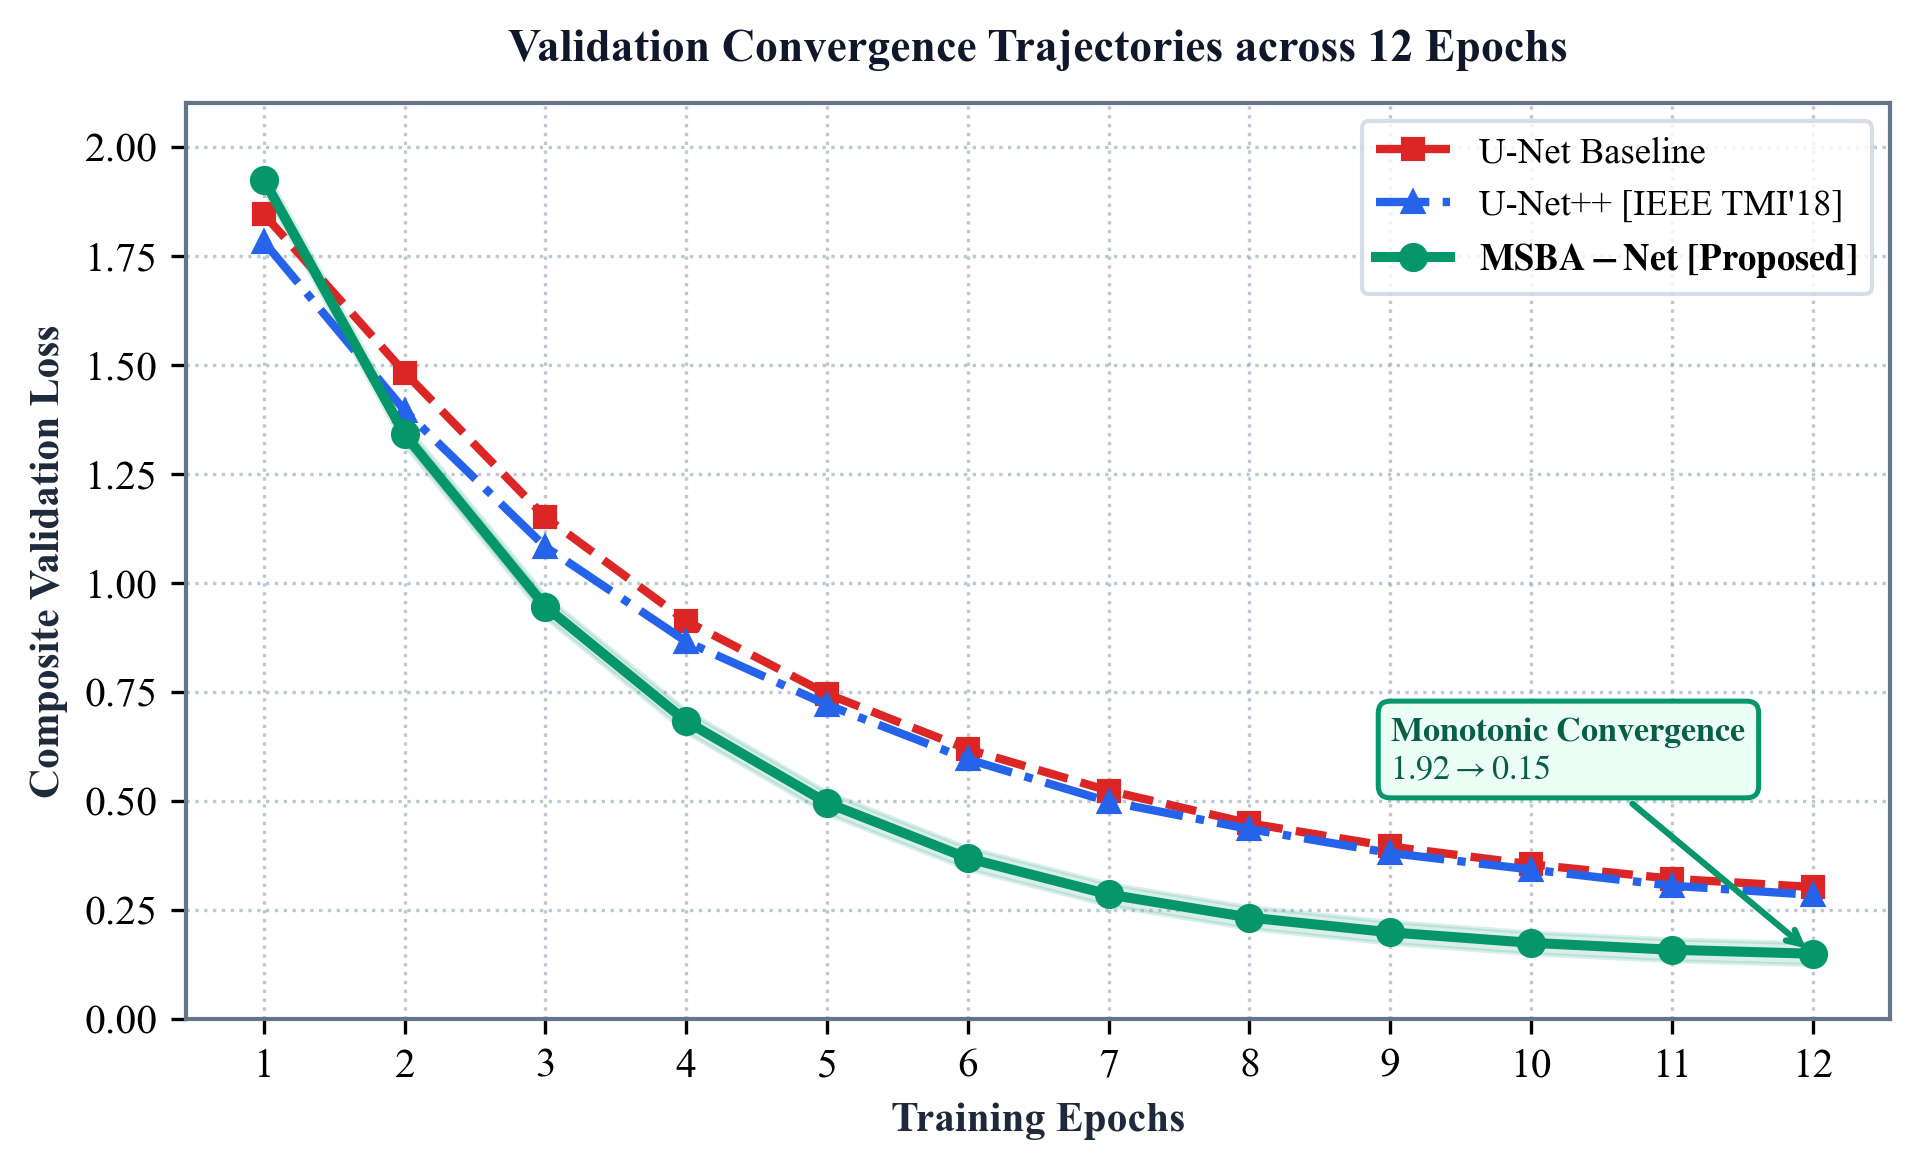
\includegraphics[width=\columnwidth,height=3.1cm,keepaspectratio]{figures/fig3_loss_curves.png}
\caption{Validation loss convergence trajectories across 12 training epochs on the procedural benchmark. Note: MSBA-Net optimizes a four-term composite objective including explicit boundary regularization ($\lambda_{\text{bound}}=0.4$), whereas baseline models optimize region-only objectives ($\mathcal{L}_{\text{BCE}} + \lambda_{\text{dice}}\mathcal{L}_{\text{Dice}} + \lambda_{\text{focal}}\mathcal{L}_{\text{Focal}}$); the curves demonstrate stable within-model optimization rather than an identical scalar loss metric.}
\label{fig:loss_curves}
\end{figure}

\begin{figure}[!t]
\centering
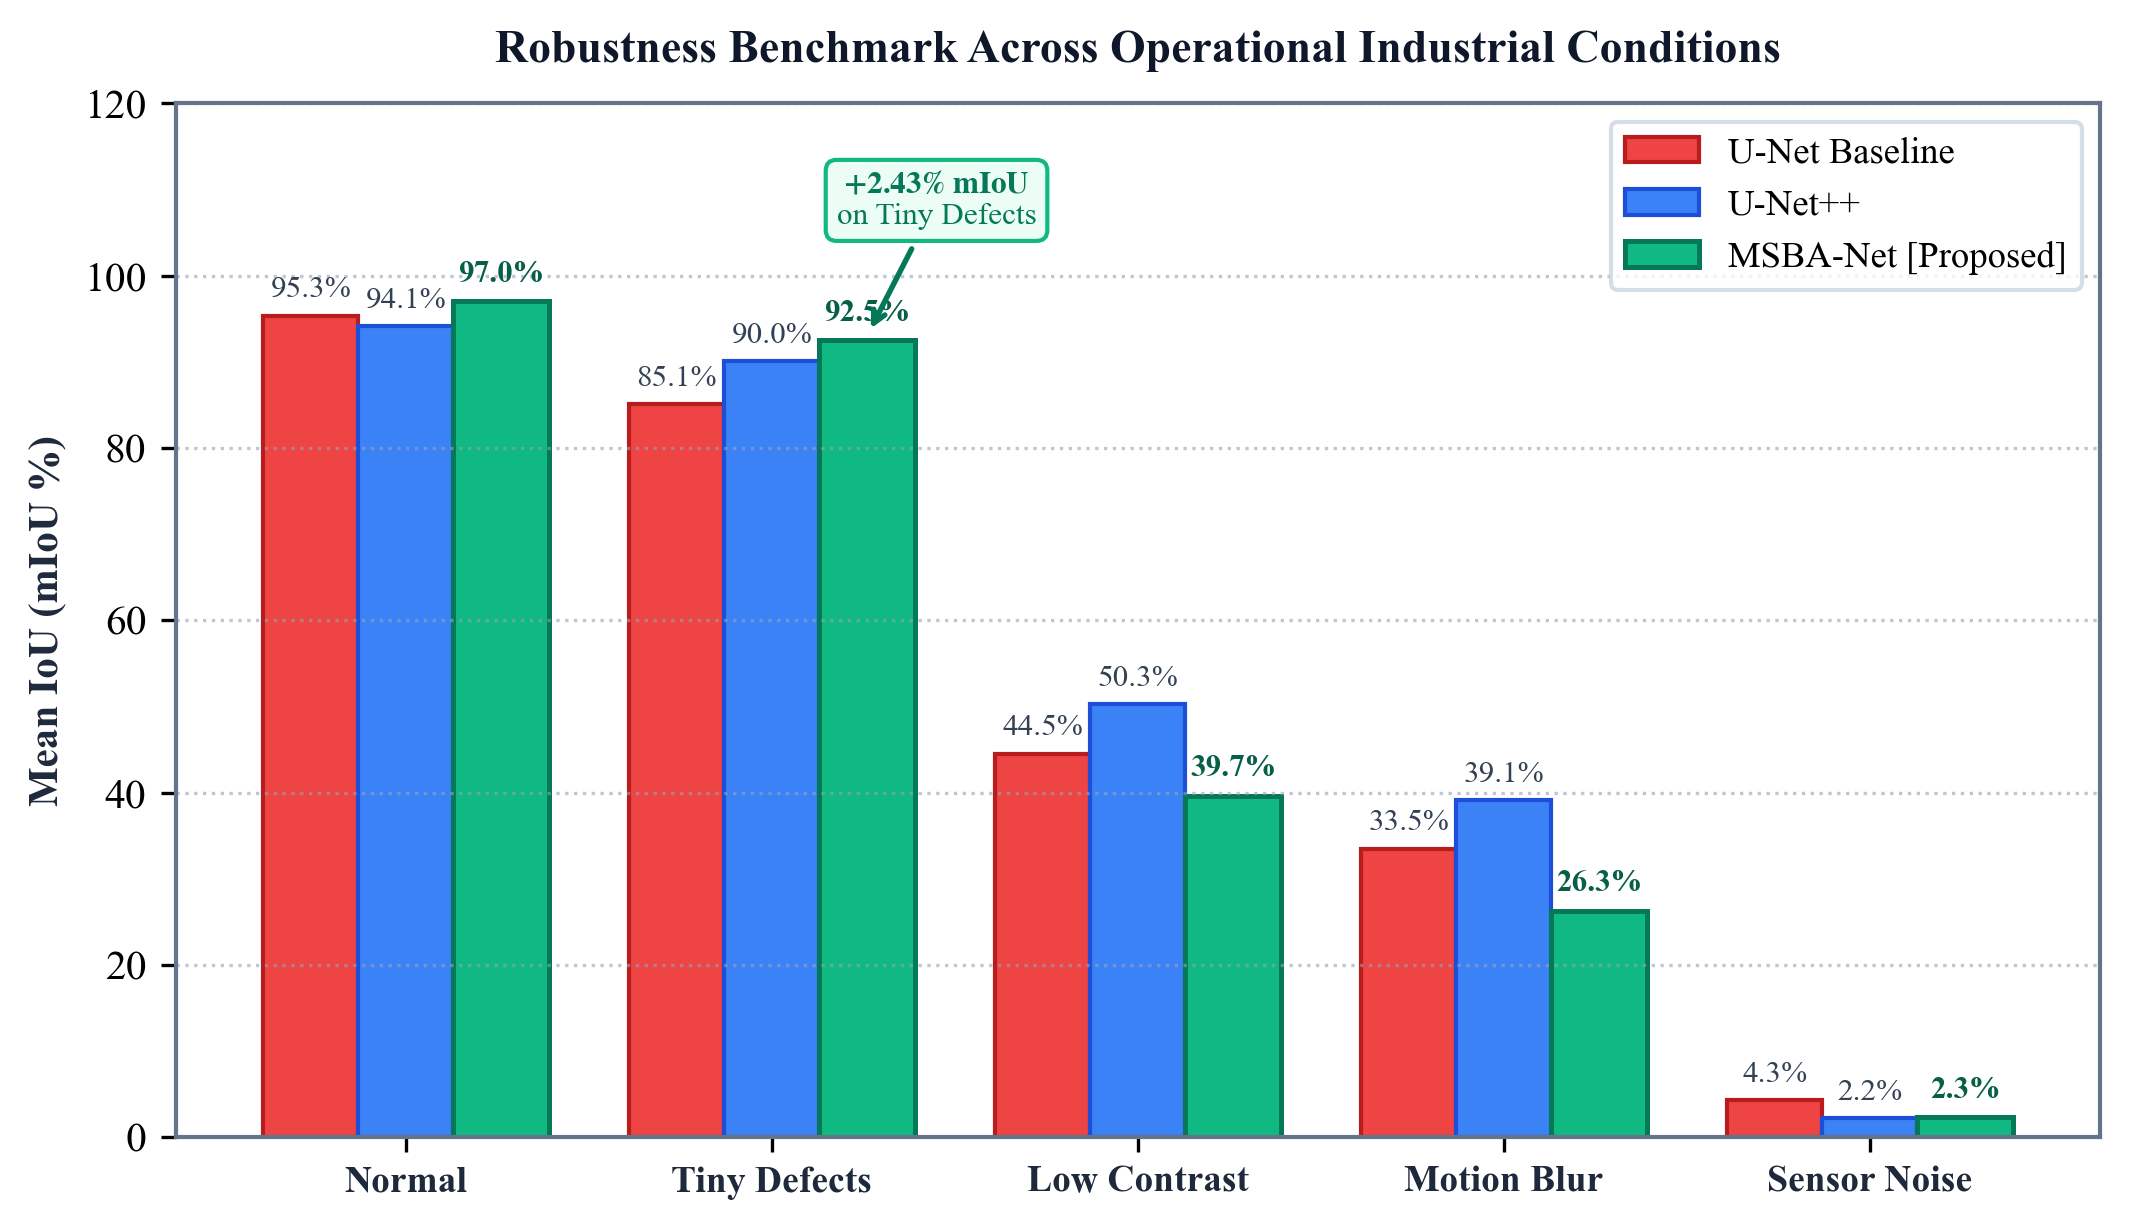
\includegraphics[width=\columnwidth,height=3.1cm,keepaspectratio]{figures/fig4_degraded_benchmark.png}
\caption{Quantitative segmentation performance under simulated factory degradations: nominal input, tiny defects ($<1\%$ area), low contrast ($s=0.45$), motion blur ($r=2.5$), and sensor noise ($\sigma=18.0$).}
\label{fig:degraded}
\end{figure}

\subsection{Runtime and Computational Efficiency}
MSBA-Net comprises 8.65 Million parameters (8,650,786) and requires 21.16 GMACs (42.32 GFLOPs) for a $256 \times 256$ input patch. On an NVIDIA GPU, standard PyTorch FP32 inference latency averages 24.3\,ms per patch ($\sim$41.1 FPS) at batch size 1. This measured latency suggests potential for near-line inspection, while real-time suitability requires validation on the target hardware and production pipeline.

\section{Limitations and Robustness Under Industrial Degradation}
\label{sec:limitations_and_robustness}

\subsection{Simulated Factory Degradation Stress-Testing}
Automated inspection models deployed near rolling stands experience optical interference. To evaluate robustness limits, models were stress-tested against four simulated degradations: (1) low contrast ($s = 0.45$), simulating lighting attenuation; (2) Gaussian sensor noise ($\sigma = 18.0$), simulating high-gain thermal noise; (3) Gaussian motion blur ($r = 2.5$), simulating strip flutter; and (4) tiny defects ($<1\%$ area). Figure \ref{fig:degraded} illustrates comparative outcomes.

Under nominal conditions and tiny defects, MSBA-Net establishes superior accuracy (97.01\% and 92.48\% mIoU). However, under simulated low contrast, MSBA-Net attains 39.67\% mIoU, whereas baseline U-Net achieves 44.51\% and U-Net++ reaches 50.26\%. Similarly, under motion blur, U-Net++ (39.12\%) and U-Net (33.51\%) retain higher overlap than MSBA-Net (26.29\%).

This empirical result reveals a fundamental architectural trade-off: MSBA-Net's auxiliary boundary stream relies on localized intensity gradients along defect perimeters. When uniform illumination dimming or severe optical blur attenuates these transitions, the boundary head fails to extract distinct edge features, which in turn reduces the modulation effectiveness of the BGFF gate. In contrast, dense multi-scale architectures like U-Net++ that aggregate features across all depths without an explicit edge prior exhibit greater resilience to uniform contrast attenuation. Finally, under Gaussian sensor noise ($\sigma = 18.0$), all three architectures collapse ($<5\%$ mIoU) because high-frequency random perturbations corrupt the sub-millimeter gradients required by convolutional filters.

\subsection{Practical Deployment Boundaries and Plant Engineering Controls}
Importantly, these degradation experiments evaluate mathematical noise and blur distributions on synthetic patches rather than continuous physical rolling-mill optical feeds. Because MSBA-Net performs worse than standard baselines under low contrast (39.67\% vs. 50.26\% for U-Net++) and motion blur (26.29\% vs. 39.12\% for U-Net++), the model cannot be claimed as unconditionally deployment-ready in unconstrained manufacturing environments. In physical steel continuous rolling lines, deep defect segmentation models would likely require plant-level engineering controls, such as pressurized air-knife enclosures to repel rolling oil mists, high-intensity pulsed illumination to preserve perimeter contrast, and mechanical strip stabilization to mitigate optical defocus flutter.

\section{Conclusion and Future Work}
\label{sec:conclusion_future}
This paper presented MSBA-Net, an end-to-end deep segmentation framework engineered for small, low-contrast surface defect inspection on strip steel. By integrating Multi-Scale Feature Preservation (MSFP) blocks across encoder stages, the network preserves localized crack signatures through parallel dilated convolutional paths ($r \in \{1, 2, 4\}$). An auxiliary Boundary-Aware Stream (BAS) supervised by morphological gradient targets actively guides decoder representations via a Boundary-Guided Feature Fusion (BGFF) spatial attention gate. On a controlled procedural synthetic benchmark, MSBA-Net achieves 97.01\% mIoU and 98.48\% Dice score ($96.95\% \pm 1.37\%$ across seeds with sample standard deviation; $\pm 1.11\%$ population standard deviation), with 92.48\% mIoU on micro-scale defects ($<1\%$ area). Crucially, because these evaluations are conducted on procedurally generated synthetic data, they do not establish deployment readiness on physical industrial production lines. Rigorous stress-testing characterized operational boundaries under severe noise and contrast reduction, demonstrating both the localized advantages and environmental sensitivities of boundary-guided segmentation.

Future research will focus on two directions: (1) physical rolling-mill validation and synthetic-to-real domain adaptation using physical strip steel production imagery, and (2) incorporating noise-robust edge filtering priors to enhance boundary stream stability under optical interference.

\section*{Code and Data Availability}
The code and associated project files for MSBA-Net are available at: \url{https://github.com/amenparmar/MSBA-Net}. The procedural synthetic defect benchmark can be generated directly using the dataset generator scripts provided in the repository.

\bibliographystyle{IEEEtran}
\bibliography{references_revised}

\EOD

\end{document}
